\documentclass[border=8pt]{standalone}
\usepackage[T1]{fontenc}\usepackage{helvet}\renewcommand{\familydefault}{\sfdefault}
\usepackage{tikz}\usetikzlibrary{arrows.meta, positioning, calc, backgrounds}
\definecolor{ink}{HTML}{1a1916}
\definecolor{inktwo}{HTML}{3a3a35}
\definecolor{inkthree}{HTML}{6a6862}
\definecolor{rule}{HTML}{b8b09a}
\definecolor{amber}{HTML}{a8730a}
\definecolor{red}{HTML}{c8261a}
\definecolor{paper}{HTML}{f0eee5}
\definecolor{slab}{HTML}{d8d4c6}
\tikzset{
  >={Stealth[length=2.2mm]},
  wire/.style={line width=0.8pt, ink},
  modwire/.style={line width=0.6pt, dashed, ink},
  tastewire/.style={line width=0.6pt, dashed, amber},
  gatewire/.style={line width=0.6pt, dotted, ink},
  block/.style={rectangle, draw=ink, line width=0.9pt, fill=slab, minimum width=3.0cm, minimum height=1.9cm, inner sep=0pt},
  perf/.style={rectangle, draw=ink, line width=0.7pt, minimum width=3.0cm, minimum height=0.7cm, inner sep=2pt, font=\footnotesize, text=ink},
  title/.style={font=\scriptsize\bfseries, text=ink, anchor=north, inner sep=2pt},
  jack/.style={circle, draw=ink, fill=paper, line width=0.5pt, minimum size=3.2pt, inner sep=0pt},
  plabel/.style={font=\tiny, text=inktwo, anchor=west, inner sep=1pt},
  olabel/.style={font=\tiny, text=inktwo, anchor=east, inner sep=1pt},
  settings/.style={font=\scriptsize, text=ink, align=left, anchor=north west, inner sep=1pt, text width=2.9cm},
}
\begin{document}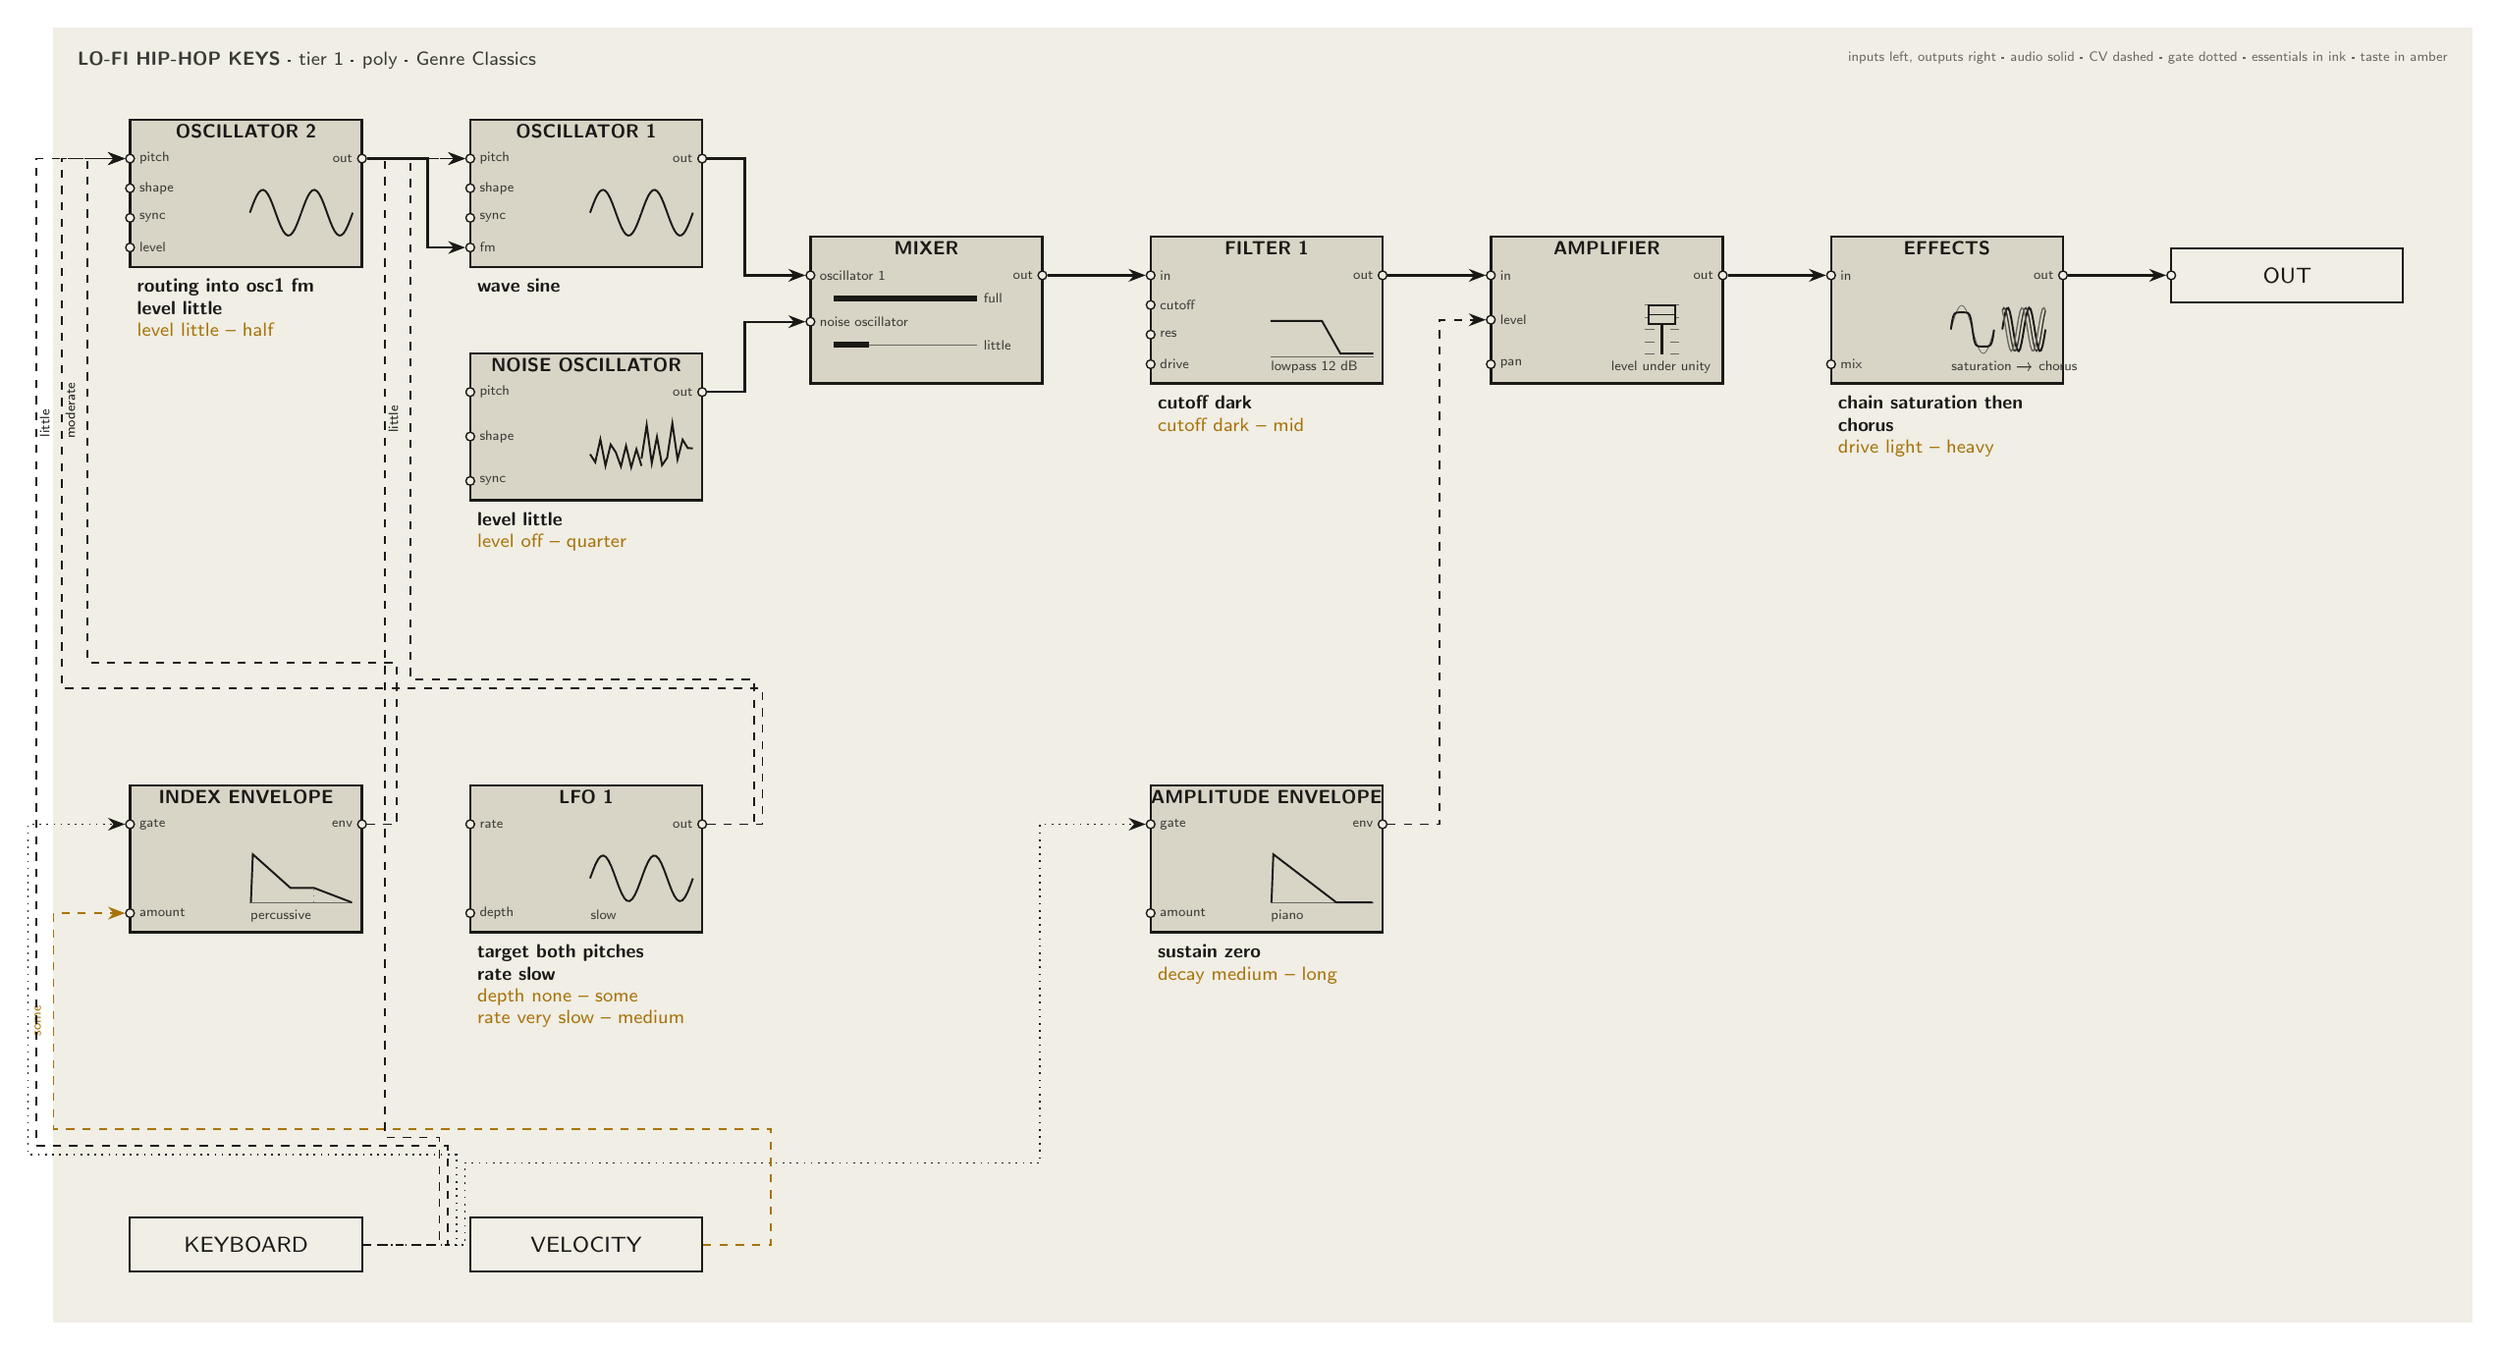
\begin{tikzpicture}
\begin{scope}[on background layer]\fill[paper] (-2.5,-13.09) rectangle (28.8,3.66);\end{scope}
\node[block, minimum height=1.9cm] (osc1) at (4.4,1.51) {};
\node[title] at (osc1.north) {OSCILLATOR 1};
\node[jack] (osc1-pitch) at (2.9000000000000004,1.96) {};
\node[plabel] at (2.9800000000000004,1.96) {pitch};
\node[jack] (osc1-shape) at (2.9000000000000004,1.5766666666666667) {};
\node[plabel] at (2.9800000000000004,1.5766666666666667) {shape};
\node[jack] (osc1-sync) at (2.9000000000000004,1.1933333333333334) {};
\node[plabel] at (2.9800000000000004,1.1933333333333334) {sync};
\node[jack] (osc1-fm) at (2.9000000000000004,0.81) {};
\node[plabel] at (2.9800000000000004,0.81) {fm};
\node[jack] (osc1-out) at (5.9,1.96) {};
\node[olabel] at (5.82,1.96) {out};
\begin{scope}
\draw[ink, line width=0.7pt] plot[domain=0.000:0.500, samples=24, variable=\u] ({4.450+\u*1.330},{0.890+(0.740)*(0.5+0.4*sin(360*(\u*2))+0.0)});
\draw[ink, line width=0.7pt] plot[domain=0.500:1.000, samples=24, variable=\u] ({4.450+\u*1.330},{0.890+(0.740)*(0.5+0.4*sin(360*(\u*2))+0.0)});
\end{scope}
\node[settings] at (2.95,0.44000000000000006) {\textbf{wave sine}};
\node[block, minimum height=1.9cm] (noise) at (4.4,-1.51) {};
\node[title] at (noise.north) {NOISE OSCILLATOR};
\node[jack] (noise-pitch) at (2.9000000000000004,-1.06) {};
\node[plabel] at (2.9800000000000004,-1.06) {pitch};
\node[jack] (noise-shape) at (2.9000000000000004,-1.635) {};
\node[plabel] at (2.9800000000000004,-1.635) {shape};
\node[jack] (noise-sync) at (2.9000000000000004,-2.21) {};
\node[plabel] at (2.9800000000000004,-2.21) {sync};
\node[jack] (noise-out) at (5.9,-1.06) {};
\node[olabel] at (5.82,-1.06) {out};
\begin{scope}
\draw[ink, line width=0.7pt] (4.450,-1.864) -- (4.517,-1.967) -- (4.583,-1.671) -- (4.649,-2.013) -- (4.716,-1.739) -- (4.783,-1.840) -- (4.849,-2.022) -- (4.915,-1.756) -- (4.982,-2.034) -- (5.049,-1.799) -- (5.115,-2.015);
\draw[ink, line width=0.7pt] (5.115,-1.922) -- (5.182,-1.486) -- (5.248,-1.981) -- (5.315,-1.639) -- (5.381,-2.006) -- (5.447,-1.910) -- (5.514,-1.465) -- (5.581,-1.932) -- (5.647,-1.676) -- (5.713,-1.784) -- (5.780,-1.788);
\end{scope}
\node[settings] at (2.95,-2.58) {\textbf{level little} \\ \textcolor{amber}{level off -- quarter}};
\node[block, minimum height=1.9cm] (osc2) at (0.0,1.51) {};
\node[title] at (osc2.north) {OSCILLATOR 2};
\node[jack] (osc2-pitch) at (-1.5,1.96) {};
\node[plabel] at (-1.42,1.96) {pitch};
\node[jack] (osc2-shape) at (-1.5,1.5766666666666667) {};
\node[plabel] at (-1.42,1.5766666666666667) {shape};
\node[jack] (osc2-sync) at (-1.5,1.1933333333333334) {};
\node[plabel] at (-1.42,1.1933333333333334) {sync};
\node[jack] (osc2-level) at (-1.5,0.81) {};
\node[plabel] at (-1.42,0.81) {level};
\node[jack] (osc2-out) at (1.5,1.96) {};
\node[olabel] at (1.42,1.96) {out};
\begin{scope}
\draw[ink, line width=0.7pt] plot[domain=0.000:0.500, samples=24, variable=\u] ({0.050+\u*1.330},{0.890+(0.740)*(0.5+0.4*sin(360*(\u*2))+0.0)});
\draw[ink, line width=0.7pt] plot[domain=0.500:1.000, samples=24, variable=\u] ({0.050+\u*1.330},{0.890+(0.740)*(0.5+0.4*sin(360*(\u*2))+0.0)});
\end{scope}
\node[settings] at (-1.45,0.44000000000000006) {\textbf{routing into osc1 fm} \\ \textbf{level little} \\ \textcolor{amber}{level little -- half}};
\node[block, minimum height=1.9cm] (mix) at (8.8,0.0) {};
\node[title] at (mix.north) {MIXER};
\node[jack] (mix-osc1) at (7.300000000000001,0.44999999999999996) {};
\node[plabel] at (7.380000000000001,0.44999999999999996) {oscillator 1};
\draw[inkthree, line width=0.3pt] (7.600,0.150) -- (9.450,0.150);
\draw[ink, line width=2.2pt] (7.600,0.150) -- (9.450,0.150);
\node[font=\tiny, text=inktwo, anchor=west, inner sep=1pt] at (9.500,0.150) {full};
\node[jack] (mix-noise) at (7.300000000000001,-0.15000000000000002) {};
\node[plabel] at (7.380000000000001,-0.15000000000000002) {noise oscillator};
\draw[inkthree, line width=0.3pt] (7.600,-0.450) -- (9.450,-0.450);
\draw[ink, line width=2.2pt] (7.600,-0.450) -- (8.062,-0.450);
\node[font=\tiny, text=inktwo, anchor=west, inner sep=1pt] at (9.500,-0.450) {little};
\node[jack] (mix-out) at (10.3,0.44999999999999996) {};
\node[olabel] at (10.22,0.44999999999999996) {out};
\node[block, minimum height=1.9cm] (filter1) at (13.200000000000001,0.0) {};
\node[title] at (filter1.north) {FILTER 1};
\node[jack] (filter1-in) at (11.700000000000001,0.44999999999999996) {};
\node[plabel] at (11.780000000000001,0.44999999999999996) {in};
\node[jack] (filter1-cutoff) at (11.700000000000001,0.06666666666666665) {};
\node[plabel] at (11.780000000000001,0.06666666666666665) {cutoff};
\node[jack] (filter1-res) at (11.700000000000001,-0.31666666666666665) {};
\node[plabel] at (11.780000000000001,-0.31666666666666665) {res};
\node[jack] (filter1-drive) at (11.700000000000001,-0.7) {};
\node[plabel] at (11.780000000000001,-0.7) {drive};
\node[jack] (filter1-out) at (14.700000000000001,0.44999999999999996) {};
\node[olabel] at (14.620000000000001,0.44999999999999996) {out};
\begin{scope}
\draw[inkthree, line width=0.3pt] (13.250,-0.605) -- (14.580,-0.605);
\draw[ink, line width=0.7pt] (13.250,-0.139) -- (13.915,-0.139) -- (14.154,-0.561) -- (14.580,-0.561);
\node[font=\tiny, text=inktwo, anchor=north west, inner sep=0pt] at (13.250,-0.650) {lowpass 12 dB};
\end{scope}
\node[settings] at (11.750000000000002,-1.0699999999999998) {\textbf{cutoff dark} \\ \textcolor{amber}{cutoff dark -- mid}};
\node[block, minimum height=1.9cm] (amp) at (17.6,0.0) {};
\node[title] at (amp.north) {AMPLIFIER};
\node[jack] (amp-in) at (16.1,0.44999999999999996) {};
\node[plabel] at (16.18,0.44999999999999996) {in};
\node[jack] (amp-level) at (16.1,-0.125) {};
\node[plabel] at (16.18,-0.125) {level};
\node[jack] (amp-pan) at (16.1,-0.7) {};
\node[plabel] at (16.18,-0.7) {pan};
\node[jack] (amp-out) at (19.1,0.44999999999999996) {};
\node[olabel] at (19.020000000000003,0.44999999999999996) {out};
\begin{scope}
\draw[ink, line width=1.2pt] (18.315,-0.570) -- (18.315,0.070);
\draw[inkthree, line width=0.3pt] (18.095,-0.570) -- (18.215,-0.570) (18.415,-0.570) -- (18.535,-0.570);
\draw[inkthree, line width=0.3pt] (18.095,-0.410) -- (18.215,-0.410) (18.415,-0.410) -- (18.535,-0.410);
\draw[inkthree, line width=0.3pt] (18.095,-0.250) -- (18.215,-0.250) (18.415,-0.250) -- (18.535,-0.250);
\draw[inkthree, line width=0.3pt] (18.095,-0.090) -- (18.215,-0.090) (18.415,-0.090) -- (18.535,-0.090);
\draw[inkthree, line width=0.3pt] (18.095,0.070) -- (18.215,0.070) (18.415,0.070) -- (18.535,0.070);
\fill[slab, draw=ink, line width=0.6pt] (18.145,-0.178) rectangle (18.485,0.062);
\draw[ink, line width=0.5pt] (18.145,-0.058) -- (18.485,-0.058);
\node[font=\tiny, text=inktwo, anchor=north west, inner sep=0pt] at (17.650,-0.650) {level under unity};
\end{scope}
\node[block, minimum height=1.9cm] (fx) at (22.0,0.0) {};
\node[title] at (fx.north) {EFFECTS};
\node[jack] (fx-in) at (20.5,0.44999999999999996) {};
\node[plabel] at (20.58,0.44999999999999996) {in};
\node[jack] (fx-mix) at (20.5,-0.7) {};
\node[plabel] at (20.58,-0.7) {mix};
\node[jack] (fx-out) at (23.5,0.44999999999999996) {};
\node[olabel] at (23.42,0.44999999999999996) {out};
\begin{scope}
\draw[inkthree, line width=0.3pt] plot[domain=0.000:0.420, samples=30, variable=\u] ({22.050+\u*1.330},{-0.620+(0.740)*(0.5+0.42*sin(360*((\u-0.000)/0.420)))});
\draw[ink, line width=0.7pt] plot[domain=0.000:0.420, samples=40, variable=\u] ({22.050+\u*1.330},{-0.620+(0.740)*(0.5+0.3*tanh(3*sin(360*((\u-0.000)/0.420))))});
\draw[ink, line width=0.7pt] plot[domain=0.500:0.920, samples=30, variable=\u] ({22.050+\u*1.330},{-0.620+(0.740)*(0.5+0.38*sin(360*((\u-0.500)/0.420)*2+0))});
\draw[inktwo, line width=0.5pt] plot[domain=0.500:0.920, samples=30, variable=\u] ({22.050+\u*1.330},{-0.620+(0.740)*(0.5+0.38*sin(360*((\u-0.500)/0.420)*2+60))});
\draw[inkthree, line width=0.5pt] plot[domain=0.500:0.920, samples=30, variable=\u] ({22.050+\u*1.330},{-0.620+(0.740)*(0.5+0.38*sin(360*((\u-0.500)/0.420)*2+120))});
\node[font=\tiny, text=inktwo, anchor=north west, inner sep=0pt] at (22.050,-0.650) {saturation → chorus};
\end{scope}
\node[settings] at (20.55,-1.0699999999999998) {\textbf{chain saturation then chorus} \\ \textcolor{amber}{drive light -- heavy}};
\node[block, minimum height=1.9cm] (menv) at (0.0,-7.1000000000000005) {};
\node[title] at (menv.north) {INDEX ENVELOPE};
\node[jack] (menv-gate) at (-1.5,-6.65) {};
\node[plabel] at (-1.42,-6.65) {gate};
\node[jack] (menv-amount) at (-1.5,-7.800000000000001) {};
\node[plabel] at (-1.42,-7.800000000000001) {amount};
\node[jack] (menv-out) at (1.5,-6.65) {};
\node[olabel] at (1.42,-6.65) {env};
\begin{scope}
\draw[inkthree, line width=0.3pt] (0.050,-7.661) -- (1.380,-7.661);
\draw[ink, line width=0.7pt] (0.063,-7.661) -- (0.088,-7.039) -- (0.575,-7.474) -- (0.879,-7.474) -- (1.367,-7.661);
\draw[inkthree, line width=0.3pt, dotted] (0.879,-7.661) -- (0.879,-7.474);
\node[font=\tiny, text=inktwo, anchor=north west, inner sep=0pt] at (0.050,-7.750) {percussive};
\end{scope}
\node[block, minimum height=1.9cm] (lfo1) at (4.4,-7.1000000000000005) {};
\node[title] at (lfo1.north) {LFO 1};
\node[jack] (lfo1-rate) at (2.9000000000000004,-6.65) {};
\node[plabel] at (2.9800000000000004,-6.65) {rate};
\node[jack] (lfo1-depth) at (2.9000000000000004,-7.800000000000001) {};
\node[plabel] at (2.9800000000000004,-7.800000000000001) {depth};
\node[jack] (lfo1-out) at (5.9,-6.65) {};
\node[olabel] at (5.82,-6.65) {out};
\begin{scope}
\draw[ink, line width=0.7pt] plot[domain=0:1, samples=40, variable=\u] ({4.450+\u*1.330},{-7.720+(0.740)*(0.5+0.4*sin(360*\u*2))});
\node[font=\tiny, text=inktwo, anchor=north west, inner sep=0pt] at (4.450,-7.750) {slow};
\end{scope}
\node[settings] at (2.95,-8.17) {\textbf{target both pitches} \\ \textbf{rate slow} \\ \textcolor{amber}{depth none -- some} \\ \textcolor{amber}{rate very slow -- medium}};
\node[block, minimum height=1.9cm] (aenv) at (13.200000000000001,-7.1000000000000005) {};
\node[title] at (aenv.north) {AMPLITUDE ENVELOPE};
\node[jack] (aenv-gate) at (11.700000000000001,-6.65) {};
\node[plabel] at (11.780000000000001,-6.65) {gate};
\node[jack] (aenv-amount) at (11.700000000000001,-7.800000000000001) {};
\node[plabel] at (11.780000000000001,-7.800000000000001) {amount};
\node[jack] (aenv-out) at (14.700000000000001,-6.65) {};
\node[olabel] at (14.620000000000001,-6.65) {env};
\begin{scope}
\draw[inkthree, line width=0.3pt] (13.250,-7.661) -- (14.580,-7.661);
\draw[ink, line width=0.7pt] (13.263,-7.661) -- (13.287,-7.039) -- (14.101,-7.661) -- (14.101,-7.661) -- (14.567,-7.661);
\node[font=\tiny, text=inktwo, anchor=north west, inner sep=0pt] at (13.250,-7.750) {piano};
\end{scope}
\node[settings] at (11.750000000000002,-8.17) {\textbf{sustain zero} \\ \textcolor{amber}{decay medium -- long}};
\node[perf] (key) at (0.0,-12.09) {KEYBOARD};
\node[perf] (vel) at (4.4,-12.09) {VELOCITY};
\node[perf, fill=paper] (out) at (26.400000000000002,0.44999999999999996) {OUT}; \node[jack] (out-in) at (24.900000000000002,0.44999999999999996) {};
\draw[wire,->] (osc2-out) -- (2.3500000000000005,1.96) -- (2.3500000000000005,0.81) -- (osc1-fm);
\draw[wire,->] (osc1-out) -- (6.45,1.96) |- (mix-osc1);
\draw[wire,->] (noise-out) -- (6.45,-1.06) |- (mix-noise);
\draw[wire,->] (mix-out) -- (filter1-in);
\draw[wire,->] (filter1-out) -- (amp-in);
\draw[wire,->] (amp-out) -- (fx-in);
\draw[wire,->] (fx-out) -- (out-in);
\draw[modwire,->] (menv-out) -- (1.95,-6.65) -- (1.95,-4.5600000000000005) -- (-2.05,-4.5600000000000005) -- (-2.05,1.96) -- (osc2-pitch);
\node[font=\tiny, text=ink, anchor=south, inner sep=1pt, rotate=90] at (-2.17,-1.3000000000000003) {moderate};
\draw[modwire,->] (aenv-out) -- (15.440000000000001,-6.65) -- (15.440000000000001,-0.125) -- (amp-level);
\draw[modwire,->] (lfo1-out) -- (6.57,-6.65) -- (6.57,-4.78) -- (2.1300000000000003,-4.78) -- (2.1300000000000003,1.96) -- (osc1-pitch);
\node[font=\tiny, text=ink, anchor=south, inner sep=1pt, rotate=90] at (2.0100000000000002,-1.4100000000000001) {little};
\draw[modwire,->] (lfo1-out) -- (6.680000000000001,-6.65) -- (6.680000000000001,-4.890000000000001) -- (-2.38,-4.890000000000001) -- (-2.38,1.96) -- (osc2-pitch);
\node[font=\tiny, text=ink, anchor=south, inner sep=1pt, rotate=90] at (-2.5,-1.4650000000000003) {little};
\draw[tastewire,->] (vel.east) -- (6.790000000000001,-12.09) -- (6.790000000000001,-10.59) -- (-2.4899999999999998,-10.59) -- (-2.4899999999999998,-7.800000000000001) -- (menv-amount);
\node[font=\tiny, text=amber, anchor=south, inner sep=1pt, rotate=90] at (-2.61,-9.195) {some};
\draw[modwire,->] (key.east) -- (2.5,-12.09) -- (2.5,-10.700000000000001) -- (1.8000000000000005,-10.700000000000001) -- (1.8000000000000005,1.96) -- (osc1-pitch);
\draw[modwire,->] (key.east) -- (2.61,-12.09) -- (2.61,-10.81) -- (-2.71,-10.81) -- (-2.71,1.96) -- (osc2-pitch);
\draw[gatewire,->] (key.east) -- (2.7199999999999998,-12.09) -- (2.7199999999999998,-10.92) -- (-2.82,-10.92) -- (-2.82,-6.65) -- (menv-gate);
\draw[gatewire,->] (key.east) -- (2.83,-12.09) -- (2.83,-11.030000000000001) -- (10.27,-11.030000000000001) -- (10.27,-6.65) -- (aenv-gate);
\node[anchor=north west, font=\scriptsize, text=inktwo] at (-2.3,3.46) {\textbf{LO-FI HIP-HOP KEYS} · tier 1 · poly · Genre Classics};
\node[anchor=north east, font=\tiny, text=inkthree] at (28.6,3.46) {inputs left, outputs right · audio solid · CV dashed · gate dotted · essentials in ink · taste in amber};
\end{tikzpicture}\end{document}
